% =============================================================
% Annexure E: Code for GLM Benchmark
% =============================================================
\section{Code for GLM Benchmark}
\label{annexure:glm_benchmark}

% -------------------------------------------------------------
\subsection{GLM Fitting via \texttt{statsmodels}}
\label{annexure:glm_fit}

\begin{lstlisting}[caption={GLM (Gamma, log-link) fitting.}]
import statsmodels.api as sm
import numpy as np

# Add intercept column
X_glm_train = sm.add_constant(X_train_raw)
X_glm_val   = sm.add_constant(X_val_raw)
X_glm_test  = sm.add_constant(X_test_raw)

# Fit GLM with Gamma family and log link
glm_model = sm.GLM(
    y_train_raw,
    X_glm_train,
    family=sm.families.Gamma(
        sm.families.links.Log())
).fit()

# Predictions on all three partitions
glm_pred_train = glm_model.predict(X_glm_train)
glm_pred_val   = glm_model.predict(X_glm_val)
glm_pred_test  = glm_model.predict(X_glm_test)
\end{lstlisting}

% -------------------------------------------------------------
\subsection{Coefficient Table Extraction}
\label{annexure:glm_coefs}

\begin{lstlisting}[caption={GLM coefficient table extraction.}]
import pandas as pd

glm_coef = pd.DataFrame({
    'Feature': ['const'] + FEATURES,
    'Coefficient': glm_model.params,
    'exp(Coef)': np.exp(glm_model.params),
    'Std Error': glm_model.bse,
    'z-value': glm_model.tvalues,
    'p-value': glm_model.pvalues
})
glm_coef['Significant (p<0.05)'] = (
    glm_coef['p-value'] < 0.05)

n_sig = glm_coef['Significant (p<0.05)'].sum()
print(f'{n_sig} of {len(glm_coef)} coefficients '
      f'are significant (p < 0.05).')
\end{lstlisting}

% -------------------------------------------------------------
\subsection{Comparison Metrics Computation}
\label{annexure:glm_metrics}

\begin{lstlisting}[caption={\texttt{compute\_metrics}: $R^2$, RMSE and MAE on the original Rand scale.}]
def compute_metrics(y_true, y_pred):
    """Compute R2, RMSE and MAE."""
    ss_res = np.sum((y_true - y_pred) ** 2)
    ss_tot = np.sum((y_true - y_true.mean()) ** 2)
    r2 = 1 - ss_res / ss_tot if ss_tot > 0 else 0.0
    rmse = np.sqrt(np.mean((y_true - y_pred) ** 2))
    mae = np.mean(np.abs(y_true - y_pred))
    return {'R2': float(r2),
            'RMSE': float(rmse),
            'MAE': float(mae)}
\end{lstlisting}

% -------------------------------------------------------------
\subsection{GLM vs DNN Comparison Table}
\label{annexure:glm_vs_dnn}

\begin{lstlisting}[caption={GLM vs DNN comparison table generation.}]
results = {}

# GLM metrics
results['GLM (Gamma, log-link)'] = {
    'Train': compute_metrics(
        y_train_raw, glm_pred_train),
    'Validation': compute_metrics(
        y_val_raw, glm_pred_val),
    'Test': compute_metrics(
        y_test_raw, glm_pred_test)
}

# DNN metrics (from checkpoint evaluation)
results['DNN (Funnel)'] = {
    'Train': compute_metrics(
        y_train_raw, dnn_pred_train),
    'Validation': compute_metrics(
        y_val_raw, dnn_pred_val),
    'Test': compute_metrics(
        y_test_raw, dnn_pred_test)
}

# Print comparison
model_order = ['GLM (Gamma, log-link)',
               'DNN (Funnel)']
print(f'{"Model":<25} {"Set":<12} '
      f'{"R2":>10} {"RMSE":>12} {"MAE":>12}')
for model_name in model_order:
    for set_name in ['Train', 'Validation', 'Test']:
        m = results[model_name][set_name]
        print(f'{model_name:<25} {set_name:<12} '
              f'{m["R2"]:>10.6f} '
              f'{m["RMSE"]:>12.2f} '
              f'{m["MAE"]:>12.2f}')

# Save to CSV
rows = []
for model_name in model_order:
    for set_name in ['Train', 'Validation', 'Test']:
        m = results[model_name][set_name]
        rows.append({
            'Model': model_name,
            'Set': set_name,
            'R2': round(m['R2'], 6),
            'RMSE': round(m['RMSE'], 2),
            'MAE': round(m['MAE'], 2)
        })

df_comparison = pd.DataFrame(rows)
df_comparison.to_csv(
    'glm_vs_dnn_comparison.csv', index=False)
\end{lstlisting}

\begin{figure}[H]
    \centering
    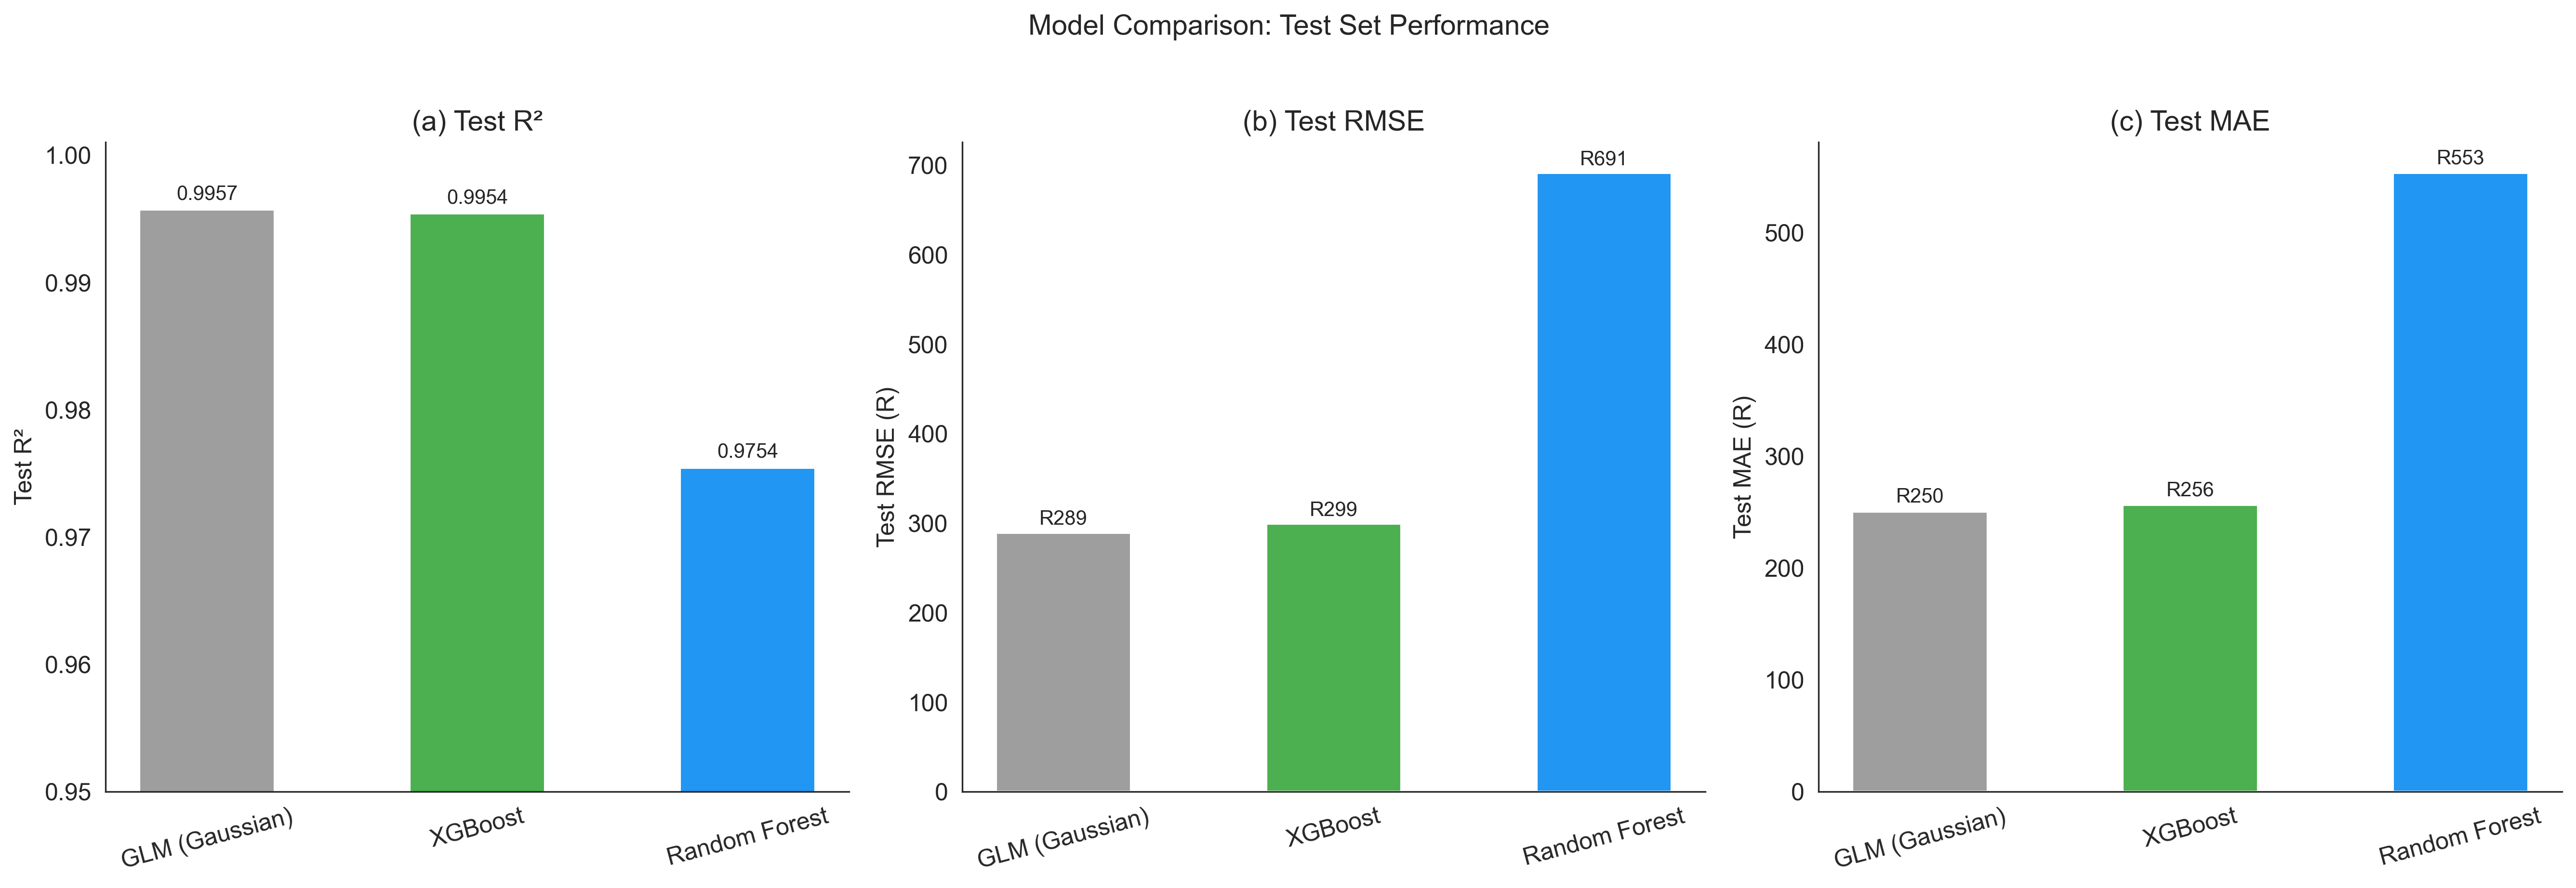
\includegraphics[width=0.9\textwidth]{Thesis/Chapter 4/Figures/fig_full_model_comparison.png}
    \caption{Full model comparison.}
    \label{fig:annexure_full_model_comparison}
\end{figure}
